%%%%%%%%%%%%%%%%%%%%%%%%
%
% $Autor: Hemanth Jadiswami Prabhakaran $
% $Datum: 2026-09-12 $
% $Pfad: GitHub/MBIDA_Thesis/report/Contents/General/en/05Methodology.tex $
% $Version: 1 $
%
% $Project: MBIDA Thesis $
%
%%%%%%%%%%%%%%%%%%%%%%%%

\chapter{Methodology}
\label{chap:methodology}

This chapter sets out the design of the empirical study: the dataset and the time windows used to train, test, and generate live forecasts (Section~\ref{sec:dataset}), the data-cleaning decisions applied before any model is fitted (Section~\ref{sec:dataPreparation}), the structure of the hierarchy the models are fitted against (Section~\ref{sec:hierarchyConstruction}), the experimental design comparing base models and reconciliation methods (Section~\ref{sec:experimentalDesign}), the evaluation framework used to score them (Section~\ref{sec:evaluationFramework}), and the limitations and fairness considerations that follow from these choices (Sections~\ref{sec:designLimitations} and~\ref{sec:fairnessNote}). The forecasting methods themselves were introduced in Chapter~\ref{chap:domainML}; their implementation is described in Chapter~\ref{chap:appDevelopment}, and the resulting accuracy figures are reported in Chapter~\ref{chap:evaluation}.

\section{Research Design}
\label{sec:researchDesign}

This thesis is structured as an empirical comparative study rather than a hypothesis-testing one: no single method combination is assumed in advance to be superior, and the research questions set out in the introduction ask how accuracy \emph{patterns} differ across hierarchy levels, base models, and volume segments, not whether one specific combination beats another at a fixed significance level. Every combination of base forecasting model and reconciliation method is fitted and evaluated under identical conditions -- the same training data, the same forecast horizon, and the same accuracy metric -- so that any differences observed can be attributed to the choice of method rather than to inconsistencies in how each was evaluated. The exploratory framing follows directly from SQ1--SQ3: each sub-question asks how a pattern changes across a dimension (hierarchy level, base model, or volume band) rather than positing a specific directional hypothesis to be confirmed or rejected.

\section{The KDD Process Framework}
\label{sec:kddFramework}

The overall pipeline is organised around the Knowledge Discovery in Databases (KDD) process \cite{Fayyad:1996}, which structures a data-driven study into five stages: selection, preprocessing, transformation, data mining, and interpretation/evaluation. Figure~\ref{fig:kddProcess} maps these five generic stages onto the concrete steps carried out in this thesis. Selection corresponds to loading the raw M5 sales and calendar files; preprocessing covers the data-cleaning decisions detailed in Section~\ref{sec:dataPreparation}; transformation covers building the complete item-store-month grid and aggregating it into the hierarchy described in Section~\ref{sec:hierarchyConstruction}; data mining covers fitting the base forecasting models and applying reconciliation (Chapter~\ref{chap:appDevelopment}); and interpretation/evaluation covers the accuracy analysis and the answers to SQ1--SQ3 (Chapter~\ref{chap:evaluation}). Using this framework keeps the two concerns of this chapter -- \emph{what} was decided and \emph{why} -- clearly separated from the \emph{how} of Chapter~\ref{chap:appDevelopment}, since each KDD stage has a single, unambiguous home in one chapter or the other.

\begin{figure}[H]
	\centering
	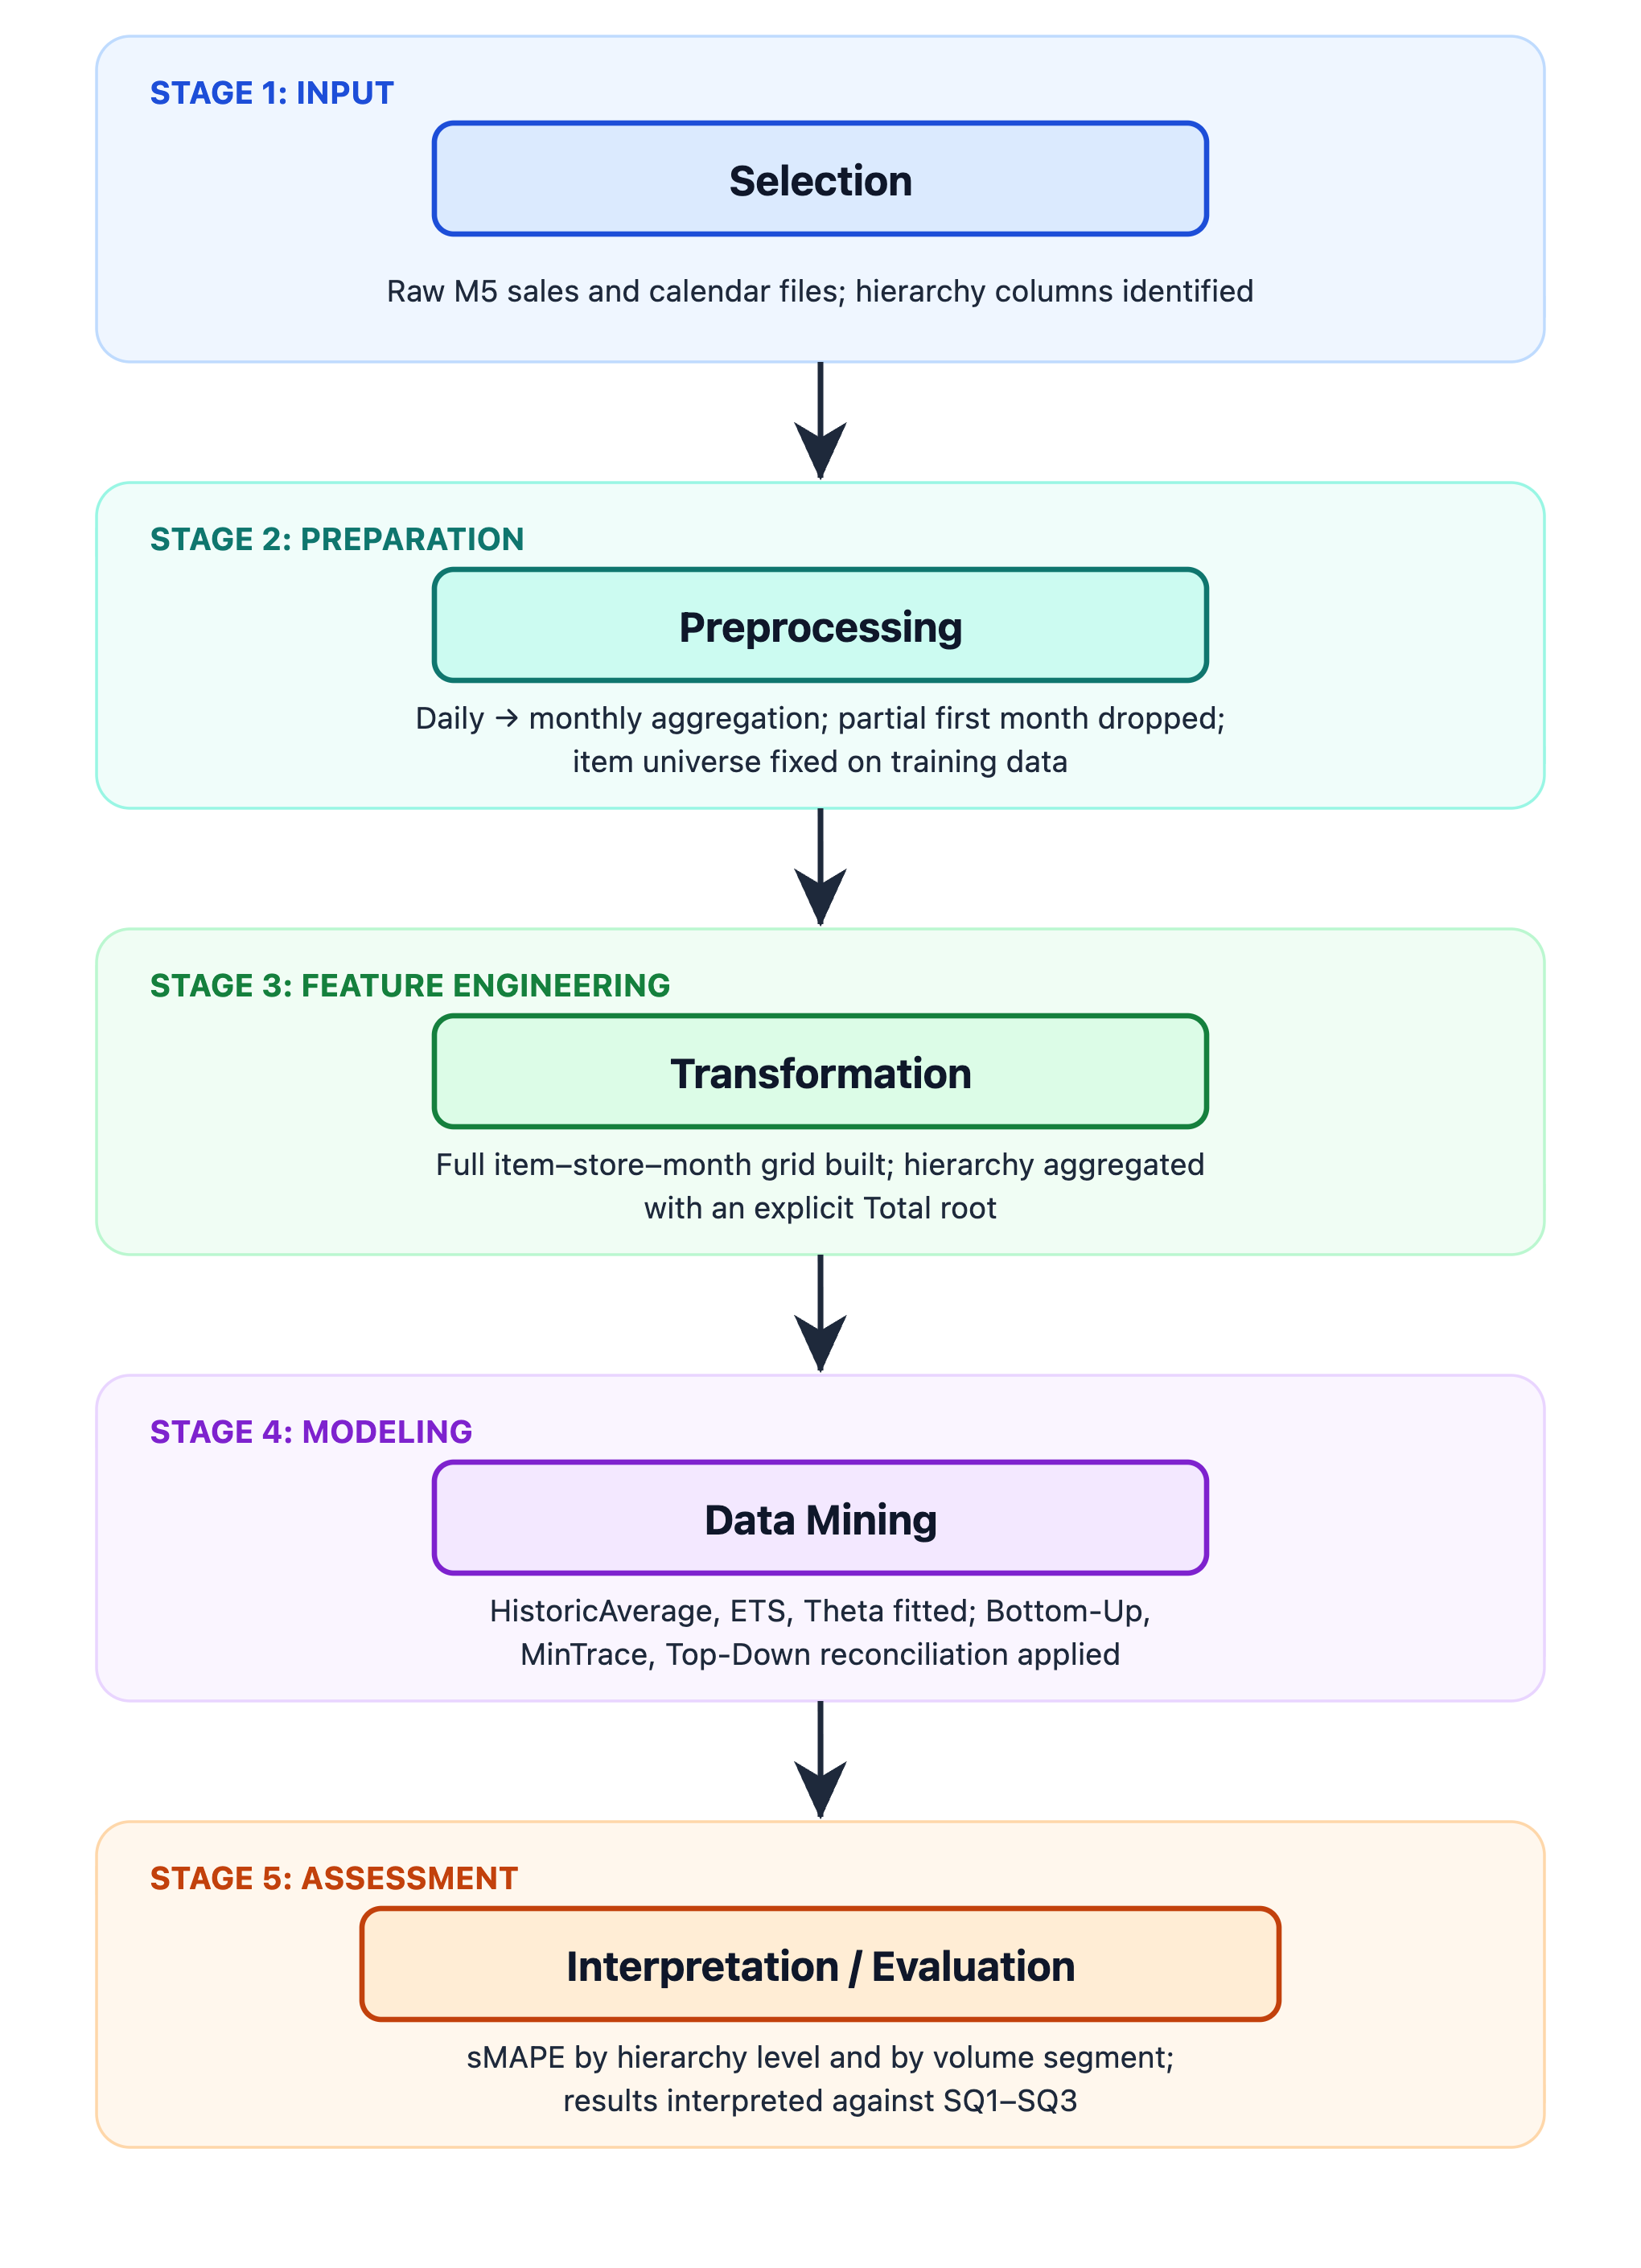
\includegraphics[width=1\linewidth]{Images/05Methodology/kddProcessDiagram}
	\caption{The five KDD process stages mapped to this thesis's own pipeline steps.}\label{fig:kddProcess}
\end{figure}


\section{Dataset}
\label{sec:dataset}

This thesis uses the M5 Forecasting -- Accuracy competition dataset \cite{Makridakis:2022}, comprising daily unit-sales records for Walmart stores across three US states. The raw sales file contains 30,490 rows, one per item-store combination, and 3,049 unique items. Each series is classified along four nested dimensions: 3 states (California, Texas, Wisconsin), 10 stores (California contributes 4, Texas and Wisconsin 3 each), 3 product categories (Foods, Hobbies, Household), and 7 departments (three within Foods, two each within Hobbies and Household). These are exactly the columns used to define the hierarchy levels in Section~\ref{sec:hierarchyConstruction}. The daily sales data itself spans 2011-01-29 to 2016-04-24 (1,913 days); an accompanying calendar file extends further, to 2016-06-19, since it also covers the competition's evaluation period, for which no actual sales figures exist in this dataset. This distinction between the calendar's date range and the sales data's actual date range is the reason the live forecast window (Section~\ref{sec:timeWindows}) needs to be described carefully rather than simply quoted from the calendar file. Figure~\ref{fig:salesByCategoryState} shows how total sales volume is distributed across these categories and states: Foods contributes roughly three times the combined volume of Household and Hobbies, and California's total sales are noticeably higher than Texas's or Wisconsin's despite the state contributing only one more store.

\begin{figure}[H]
	\centering
	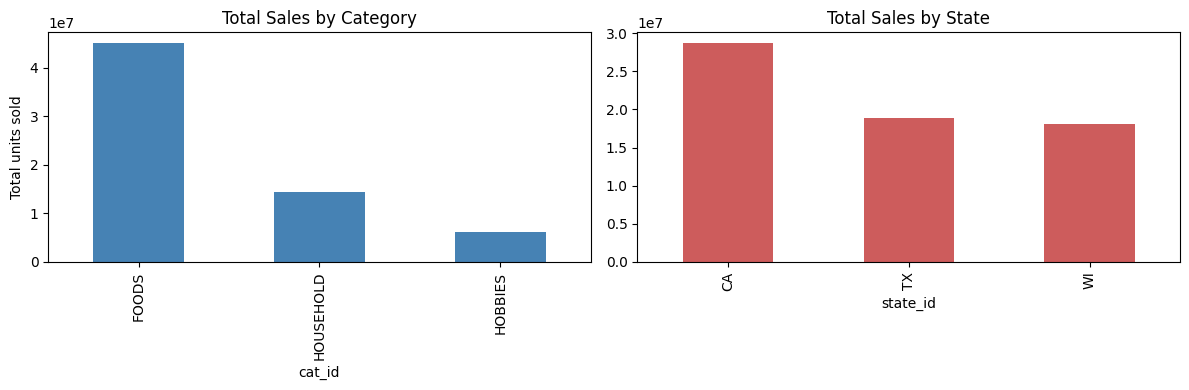
\includegraphics[width=1\textwidth]{Images/05Methodology/salesByCategoryState}
	\caption{Total training-period sales by product category and by state. Source: \texttt{01\_eda.ipynb}.}\label{fig:salesByCategoryState}
\end{figure}

\subsection{Time Windows and the Live Evaluation Period}
\label{sec:timeWindows}

Three non-overlapping periods are defined along the time axis: a training period, a test period, and a live period. Models are fitted once on the training period alone and evaluated on the immediately following test period, whose actual outcomes are known and withheld from model fitting; performance on this test period is what Chapter~\ref{chap:evaluation} reports. A second forecast, trained on the training and test periods combined, produces the live period -- this is the forecast horizon written into the dashboard described in Chapter~\ref{chap:appDeployment}. Figure~\ref{fig:timeWindows} lays out all three periods on a single timeline, since the boundaries between them do not line up neatly with where the real underlying data itself ends.

\begin{figure}[H]
	\centering
	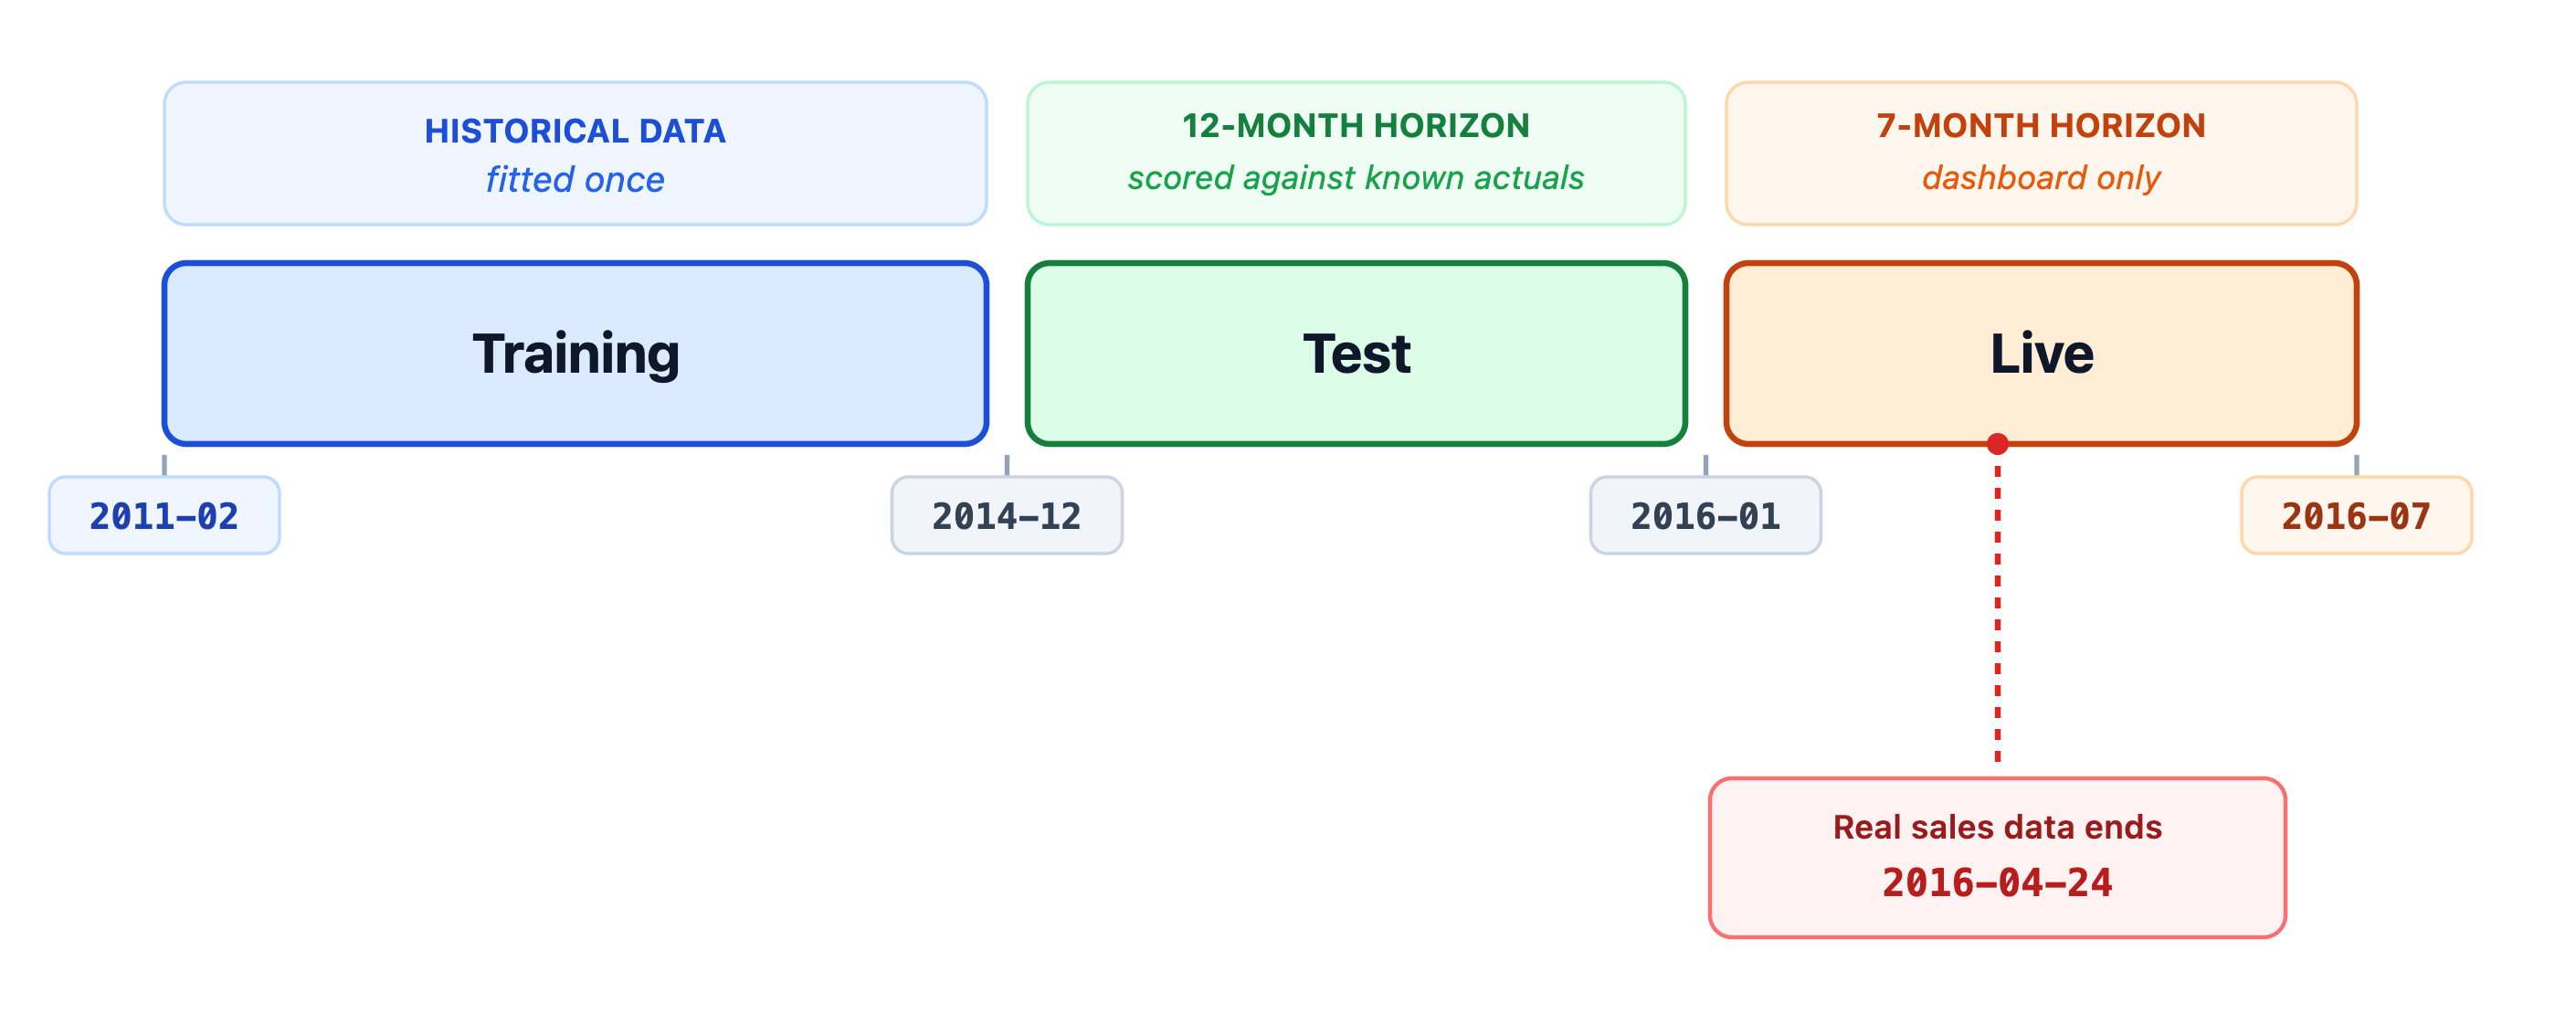
\includegraphics[width=1\linewidth]{Images/05Methodology/timeWindowsDiagram}
	\caption{The training, test, and live time windows (schematic, not to scale). The live window is trained on training and test data combined and extends three months past where real sales data actually ends.}\label{fig:timeWindows}
\end{figure}


The live period is deliberately extended to 2016-07-01, three months beyond the point at which the real sales data ends (2016-04-24). This is done purely so the dashboard has a horizon of live forecasts to display; there is no ground truth available for May, June, or July 2016 in this dataset, and the live period is consequently never used for any accuracy evaluation in this thesis, only for the deployed dashboard. Any reference to the data range in later chapters should accordingly be read as "training and test data through April 2016, with the live forecast window extended to July 2016 for the dashboard's benefit" rather than as a single continuous range of real observations running to mid-2016.

\section{Data Preparation}
\label{sec:dataPreparation}

Four cleaning decisions are applied to the raw daily data before any model is fitted, in the order presented below. This order matters: later steps depend on earlier ones having already run (for example, the item universe fixed further below is defined using monthly, not daily, sales figures).

\subsection{Daily-to-Monthly Aggregation}
\label{sec:dailyToMonthly}

At the daily, item-store level, 68.2\% of all observations record zero sales, against 0.0\% of observations at the state level, where some purchase of some product is effectively guaranteed on any given day across an entire state. This intermittency (introduced conceptually in Section~\ref{sec:intermittentDemand}) is characteristic of item-level retail demand and becomes markedly more pronounced the more granular the level of observation. Figure~\ref{fig:itemSparsity} shows this sparsity across the full item catalogue rather than as a single averaged figure: the distribution is skewed heavily toward the sparse end, with most items recording zero sales on well over half of all days, rather than clustering near zero as a small, uniform intermittency rate would suggest. Aggregating daily sales to monthly totals does not remove this sparsity, but it substantially reduces it: a month in which an item sold at all is no longer a zero observation, even if most of the individual days within it were. Temporal aggregation of this kind is a recognised trade-off in the forecasting literature more broadly: coarsening the sampling frequency of a series trades away sub-period detail in exchange for a more stable, less noisy signal to forecast from \cite{Athanasopoulos:2017}. This aggregation also matches the planning horizon most retail businesses use in practice, and it is the step from which every later part of the pipeline -- the calendar-boundary fix below, the hierarchy, and the forecasting models -- proceeds.

\begin{figure}[H]
	\centering
	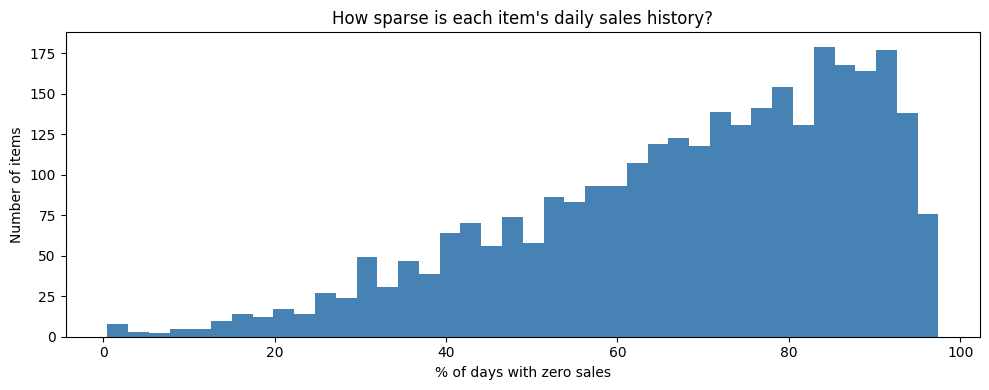
\includegraphics[width=1\textwidth]{Images/05Methodology/itemSparsityHistogram}
	\caption{Distribution across items of the percentage of days with zero sales, at the daily item-store level. Source: \texttt{01\_eda.ipynb}.}\label{fig:itemSparsity}
\end{figure}

\subsection{Dropping the Partial First Calendar Month}
\label{sec:partialFirstMonth}

Because the sales data begins on 2011-01-29, resampling to calendar months places only three real days -- 2011-01-29 through 2011-01-31 -- into the resulting 2011-01-01 monthly bucket, against a normal January's 31. That three-day bucket records 88,163 units of total sales, compared with 726,375 in the following, complete February bucket: only 12.1\% of a normal month's volume. Left in place, this heavily undercounted bucket becomes one of only four training-period Januaries available to a model configured with a 12-month seasonal period (Section~\ref{sec:seasonLength}), distorting the January seasonal index those models rely on. The partial bucket is therefore dropped before any further processing, leaving every other monthly bucket untouched.

\subsection{Fixing the Item Universe on Training Data Only}
\label{sec:itemUniverse}

Not every item was on sale for the full 2011--2016 window; some were introduced only partway through. Checking each item's monthly sales against the training/test boundary shows that 25 of the 3,049 raw items recorded no sales at all before that boundary, leaving 3,024 items with genuine training history. These 25 items are removed from the dataset entirely, because no model fitted only on training data could ever have learned a pattern for a series with no training-period observations -- forecasting them would amount to guessing rather than extrapolating. This filter is applied once, at the training boundary, before the hierarchy or the forecast grid is built, so the training, test, and live periods -- and the evaluation built on top of them -- automatically share an identical, training-consistent item universe with no later step at which their item sets could drift apart. With 10 stores and 3,024 remaining items, the bottom level of the hierarchy comprises 30,240 item-store series.

\subsection{Adding an Explicit Total Root}
\label{sec:totalRoot}

California, Texas, and Wisconsin do not contribute an equal number of stores: California has 4, Texas and Wisconsin have 3 each. Without an explicit node sitting above the state level, the hierarchy is really three separate trees, one rooted at each state, with no single top. Top-Down reconciliation (Section~\ref{subsec:topDown}) is only mathematically well defined when there is one root series to distribute downward from; without an explicit root, an implementation asked to reconcile top-down has to infer which of the three state-level series counts as "the top," typically defaulting to whichever aggregates the most bottom-level series. A single constant column, "Total," is therefore introduced above the state level, giving the hierarchy one unambiguous root and making Top-Down reconciliation well defined across the entire structure.

\section{Hierarchy Construction}
\label{sec:hierarchyConstruction}

With the Total root in place, the hierarchy used throughout this thesis has six levels: Total, State, Store, Category, Department, and Item, exactly as shown in Figure~\ref{fig:hierarchyDiagram} in the introduction. Every node belongs to exactly one parent at the level above it -- every store belongs to one state, every department instance belongs to one store and one category, and so on -- which makes this a \emph{simple tree} hierarchy in the sense introduced in Section~\ref{sec:hierarchicalCoherence}, rather than a grouped or cross-product hierarchy in which a series could be classified along more than one independent dimension at once. This distinction matters because the reconciliation methods compared in this thesis (Section~\ref{sec:reconciliationTheory}) are defined in terms of the summing matrix $S$ that a simple tree naturally produces; a cross-product hierarchy would require a different aggregation treatment not used here. Building this six-level structure over the training-consistent item universe described above yields 30,354 total series: 1 Total node, 3 State nodes, 10 Store nodes, 30 Category nodes, 70 Department nodes, and 30,240 Item-level (bottom) series.

\section{Experimental Design}
\label{sec:experimentalDesign}

The comparison at the centre of this thesis is a full factorial design \cite{Montgomery:2004} crossing three base forecasting models (HistoricAverage, ETS, Theta; Section~\ref{sec:baseModels}) with three reconciliation methods (Bottom-Up, MinTrace, Top-Down; Section~\ref{sec:reconciliationTheory}), giving nine base-model/reconciler combinations in total. Every one of these nine combinations is then evaluated along two further, independent dimensions: the six hierarchy levels defined above, and the six cumulative volume-percentile bands defined in Section~\ref{sec:volumeFramework}. Figure~\ref{fig:experimentalDesignGrid} lays out the resulting $3 \times 3 \times 6 \times 6$ design space. Implementing this design -- fitting the models and applying the reconciliation methods -- is covered in Chapter~\ref{chap:appDevelopment}; the two configuration decisions that shape every cell of this design are set out next.

\begin{figure}[H]
	\centering
	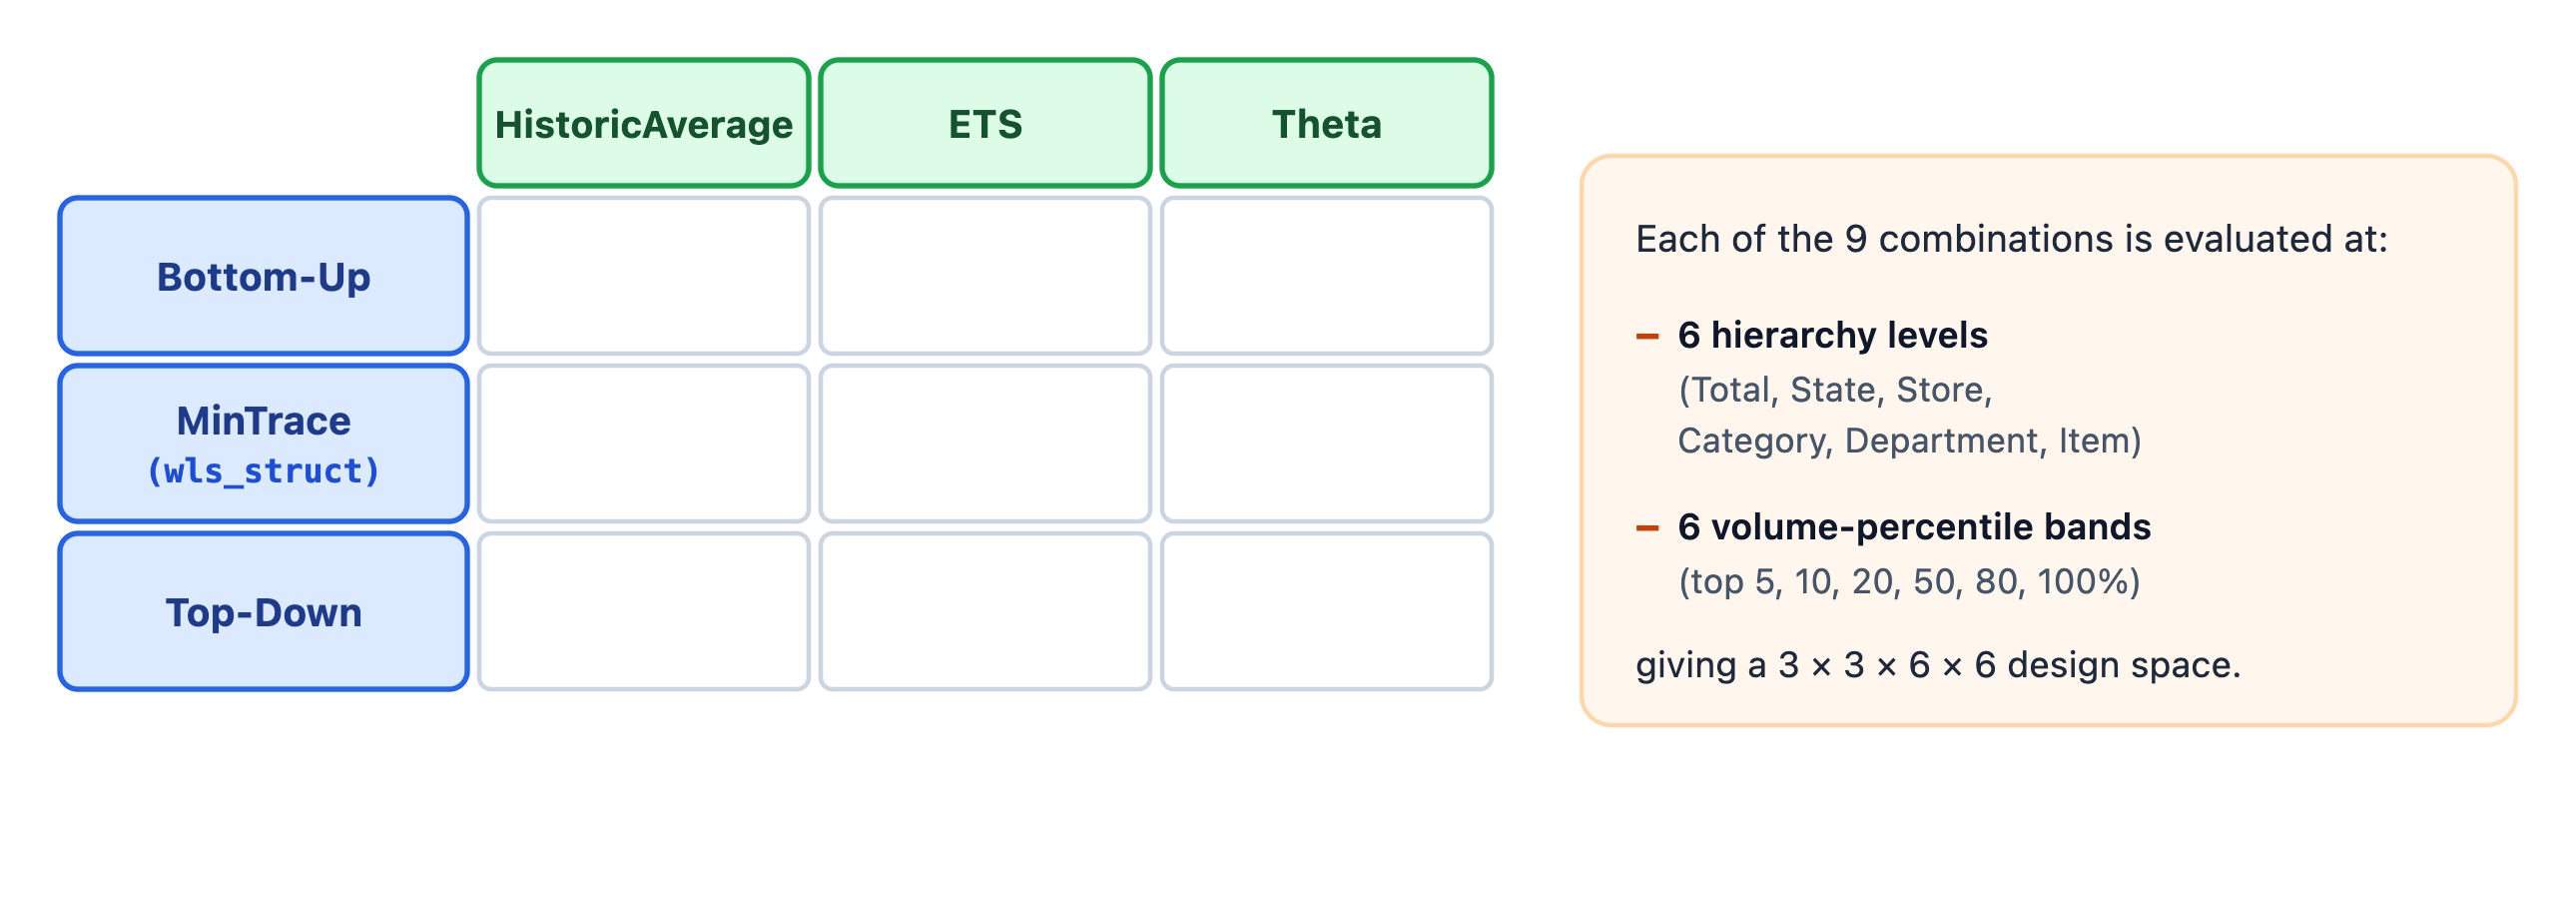
\includegraphics[width=1\linewidth]{Images/05Methodology/experimentalDesignGrid}
	\caption{The $3 \times 3$ base-model / reconciler grid; every cell is further evaluated across 6 hierarchy levels and 6 volume-percentile bands.}\label{fig:experimentalDesignGrid}
\end{figure}


\subsection{Model Configuration: A 12-Month Seasonal Period}
\label{sec:seasonLength}

Figure~\ref{fig:monthlySeasonality} plots total monthly sales across every item and store and shows a clear, repeating annual pattern, rather than a series that simply trends up or down at random. ETS and Theta both require a seasonal period to be specified when a seasonal component is used; this thesis sets that period to 12 months for both models. Without it, both models default to a seasonal period of 1 -- effectively no seasonality at all -- and produce forecasts that are close to flat, missing the recurring pattern the monthly data actually shows. HistoricAverage has no seasonal component and is unaffected by this setting.

\begin{figure}[H]
	\centering
	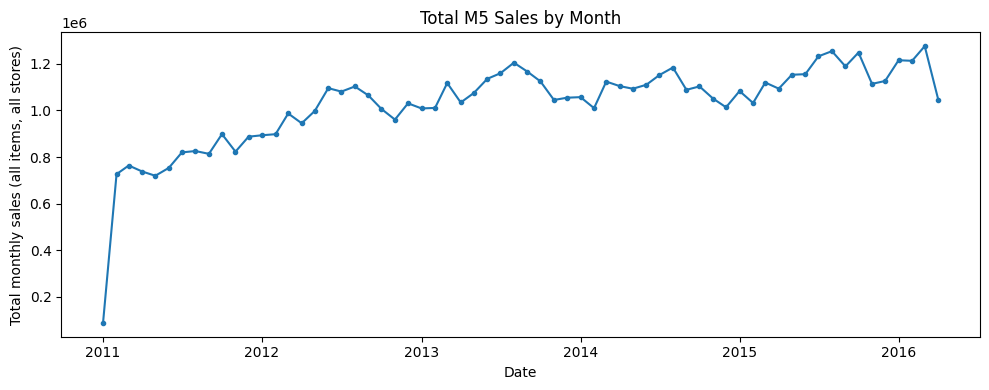
\includegraphics[width=1\textwidth]{Images/05Methodology/monthlySeasonality}
	\caption{Total monthly sales across all items and stores, 2011--2016, showing a recurring annual pattern.}\label{fig:monthlySeasonality}
\end{figure}

\subsection{Ensuring a Fair Comparison: Clipping Negative Base Forecasts}
\label{sec:clippingRationale}

Units sold cannot be negative, and the raw daily data confirms this constraint holds throughout: none of the 58,327,370 raw daily observations is negative, and the minimum observed daily value is 0. The base forecasting models, however, are not aware of this floor -- ETS and Theta are free to extrapolate a downward trend straight through zero, while HistoricAverage, as a simple mean, cannot. This asymmetry creates a risk of an unfair comparison between reconciliation methods specifically: MinTrace is configured to enforce non-negativity internally as part of its reconciliation step, while Bottom-Up simply inherits whatever value the base model produced for each bottom-level series. Comparing the two reconcilers on unclipped base forecasts would therefore partly be comparing "reconciliation with an enforced floor at zero" against "reconciliation without one," rather than comparing the reconciliation methods themselves on equal footing. Every base forecast is accordingly clipped at zero before any reconciliation method is applied, so that Bottom-Up, MinTrace, and Top-Down all start from the same, already-nonnegative base forecasts; the resulting clip counts are reported alongside the implementation in Chapter~\ref{chap:appDevelopment}.

\section{Evaluation Framework}
\label{sec:evaluationFramework}

Two evaluation lenses are applied to every combination in the design space described above: accuracy by hierarchy level, and accuracy by business volume segment. Both use the same underlying metric, defined next.

\subsection{sMAPE}
\label{sec:smape}

Accuracy throughout this thesis is measured with the symmetric Mean Absolute Percentage Error (sMAPE), chosen for its demonstrated rank stability on hierarchical retail data: across the top-performing submissions to the M5 competition, sMAPE achieves a rank-stability correlation of 0.75--0.83 between comparable dataset splits, compared with just 0.24--0.56 for the competition's own official metric, price-weighted RMSSE \cite{Hewamalage:2021} -- and its interpretability relative to scale-dependent alternatives. For a forecast $F$ and an actual value $A$,
\[
\text{sMAPE} = \operatorname{mean}\!\left( \frac{|F - A|}{|F| + |A|} \right) \times 100 .
\]
A worked example: for an actual value of 10 and a forecast of 12, the error is $|12-10|=2$ and the denominator is $|12|+|10|=22$, giving an sMAPE contribution of $2/22 \approx 9.09\%$. Where both the actual value and the forecast are zero -- a dead series correctly predicted as dead -- the ratio is defined as zero rather than left undefined, so that a perfect forecast of "no sales" is scored as a perfect forecast rather than penalised or excluded.

This thesis uses the 0--100\% scaling convention shown above, rather than the alternative 0--200\% version some textbooks define by adding a factor of two to the denominator. Neither convention is more "correct" than the other; they are simply different scalings of the same underlying idea, and using two of them side by side risks producing numbers that look comparable but are not. The 0--100\% convention is used here because it is the convention implemented directly by the sMAPE function in this thesis's forecasting toolchain (Chapter~\ref{chap:domainKnowledgeTools}), so only one scale is ever in play.

\subsection{Volume-Percentile Evaluation Framework}
\label{sec:volumeFramework}

Alongside the hierarchy-level view, forecast accuracy is evaluated separately across business-relevant volume segments, reflecting the Pareto-driven motivation introduced in Section~\ref{sec:paretoPrinciple}: a small number of series typically account for a disproportionate share of total sales, and treating every series as equally important would obscure how well a method serves the series that matter most operationally. Every bottom-level (item-store) series is ranked by its total \emph{training-period} sales volume alone -- never by test-period sales, since a real forecaster would not have access to future sales when deciding which series matter most. Walking down this ranking from the largest seller, cumulative bands are defined at 5\%, 10\%, 20\%, 50\%, 80\%, and 100\% of total training volume; each band contains whichever series, taken from the top, are needed to reach that cumulative share.

Because sales volume is highly concentrated, these bands correspond to very different numbers of series: across the 30,240 bottom-level series in this dataset, the top 5\% of training volume is covered by just 29 series (0.10\% of all series), the top 10\% by 94 series (0.31\%), the top 20\% by 326 series (1.08\%), the top 50\% by 2,151 series (7.11\%), and the top 80\% by 8,155 series (26.97\%); the top 100\% band is, by definition, all 30,240 series. "Top 5\% of volume" is therefore a statement about sales share, not about the fraction of the product catalogue it covers. This evaluation is carried out strictly at the bottom (item-store) level and is never re-aggregated into a synthetic "state" or "category" total built from only the selected series in a band, since a state built from 5\% of its items would not represent a real state-level forecast.

\section{Limitations of the Design}
\label{sec:designLimitations}

Several limitations follow from the design choices set out above. First, MinTrace is implemented throughout using structural scaling (\texttt{wls\_struct}), which weights each hierarchy node only by how many bottom-level series sum into it. The sparse implementation used in this thesis (Chapter~\ref{chap:domainKnowledgeTools}) does not offer a shrinkage-based covariance estimator; it does offer \texttt{wls\_var}, which weights each node by the variance of its in-sample forecast errors, but this requires in-sample fitted values for all 30,354 series and was not evaluated. Both variants, and Top-Down with forecast rather than historical proportions, are left as future work. Second, every finding in this thesis is drawn from a single dataset -- the M5 Walmart retail data -- and while this dataset shares key structural features with the MRO hierarchical forecasting context that motivated this thesis (Chapter~\ref{chap:introduction}), the extent to which these specific findings generalise to other domains or hierarchies is not tested here. Third, aggregating daily sales to monthly totals (Section~\ref{sec:dailyToMonthly}) trades off intra-month granularity for a more tractable, less sparse series, in line with the general temporal-aggregation trade-off noted above \cite{Athanasopoulos:2017}: any weekday effects, promotional spikes, or other sub-monthly demand patterns are smoothed away by this choice and are outside the scope of what this thesis's forecasts can capture. Fourth, all results come from a single forecast origin (one train/test split), use no exogenous drivers such as prices, promotions or events, and evaluate point forecasts only, without prediction intervals. Fifth, sMAPE is discontinuous at zero: whenever the actual value is 0, any forecast above 0 -- however small -- scores the maximum error, while only an exact 0 scores none \cite{Hyndman:2006}. At the item level, where many test months have zero sales, this makes the metric sensitive to tiny positive values. It rewards clipping negative forecasts to exactly zero, and it likely explains much of MinTrace's higher item-level error, since its non-negative optimisation can return small positive values where Bottom-Up returns zero.

\section{Fairness/Bias Note}
\label{sec:fairnessNote}

The volume-percentile framework defined above is a deliberate methodological choice, and it is worth being explicit about what it optimises for. By design, it directs evaluation attention toward the small number of high-volume series that a business would care about most, which means that accuracy on the long tail of low-volume, individually minor series is structurally given less weight in how "success" is judged throughout this thesis -- even though the results chapter shows this long tail is exactly where the gap between the base forecasting models is most pronounced. This is not a flaw to be corrected so much as a framing decision that should be read alongside the results in Chapter~\ref{chap:evaluation}: a method combination that performs well under this framework is one well suited to business-critical, high-volume forecasting, not necessarily one that serves every individual series in the catalogue equally well.